\chapter{Traffic Shaping}

%  Definizione traffic shaping generale
\section{Definizione}
\begin{defn}[Traffic Shaping]
  Il traffic shaping è una tecnica di gestione della larghezza di banda utilizzata nelle reti informatiche,
  che ritarda alcuni o tutti i datagrammi IP per adeguarli al profilo di traffico desiderato.
  Consente di migliorare le prestazioni della rete controllando in il traffico in entrata e in uscita o di simulare condizioni di reti reali.
\end{defn}
A differenza di tecniche basate sullo scarto di datagrammi IP in eccesso, il traffic shaping ne ritarda l'invio, trattendoli in una coda. \\
Esistono alcuni scenari tipici in cui è applicato:
\begin{itemize}
  \item \textbf{Limitazione} della banda per utenti e servizi in una rete;
  \item \textbf{Garanzia} di banda minima per determinati flussi;
  \item \textbf{Prioritizzazione} del traffico;
  \item \textbf{Minimizzazione} della latenza;
\end{itemize}

% Traffci shaping su Linux
\section{Traffic Shaping in Ambienti Linux}
In ambienti Linux il traffic shaping può essere effettuato con il comando \texttt{tc} (traffic control) \cite{tc}, disponibile nella suite di comandi \texttt{iproute2} \cite{iproute2}.\\
Nella pagina ufficiale del manuale di \cite{tc}, viene evidenziato come l'elaborazione del traffico è gestita tramite tre tipi di oggetti: \textbf{qdisc}, \textbf{classi} e \textbf{filtri}.

\subsection{Queueing Discipline (qdisc)}
\begin{defn}[qdisc]
  qdisc è l'abbreviazione di queueing discipline: rappresenta il meccanismo con cui il kernel gestisce l'invio dei pacchetti su un'interfaccia,
  accodandoli secondo una politica configurabile \cite{tc}.
\end{defn}
Alcune qdisc possono essere \textbf{classful}, quindi contenere classi con con a loro volta una propria qdisc, creando di fatto una gerarchia.
Il kernel può decidere di inviare un pacchetto di una classe invece che un'altra, per dare priorità a determinati tipi di traffico cercando di estrarre pacchetti prima da certe classi. \\
\vspace*{0.01\textheight}
Eventualmente, le qdisc possono essere pure \textbf{classles}, potendo solo riordinare, ritardare o scartare pacchetti.

\subsection{Token Bucket Filter (TBF)}
\begin{defn}[Token Bucket Filter]
  Disciplina di accodamento \textbf{classles} disponibile per il controllo del traffico nel comando \texttt{tc}.
  Funziona puramente da shaper e non si occupa mai dello scheduling del traffico. \cite{tc-tbf}
\end{defn}
TBF è molto leggero e non appesantisce la rete né il processore. Il suo unico limite è che può lavorare su una interfaccia usando una sola coda.

\subsubsection{Algoritmo}
L'implementazione consiste in un buffer (\textbf{bucket}) che viene costantemente riempito di gettoni (\textbf{tokens}), a una velocità specifica \textbf{rate}.
Il bucket ha un capienza (\textbf{burst}), che indica quanti gettoni può contenre al massimo. Un token equivale a circa un byte. \\ 
\vspace*{0.01\textheight}
Quando un pacchetto deve essere inviato, i gettoni necessari per inviarlo vengono rimossi dal bucket.
Nel caso non fossero sufficienti, il pacchetto viene inserito in una coda finchè non vengono generati abbastanza gettoni per inviarlo, in caso contrario viene mandato immediatamento.
Sfruttando il rate dei gettoni e il burst è possibile, quindi, ritardare l'invio dei pacchetti.

\begin{figure}[!htb]
    \centering
    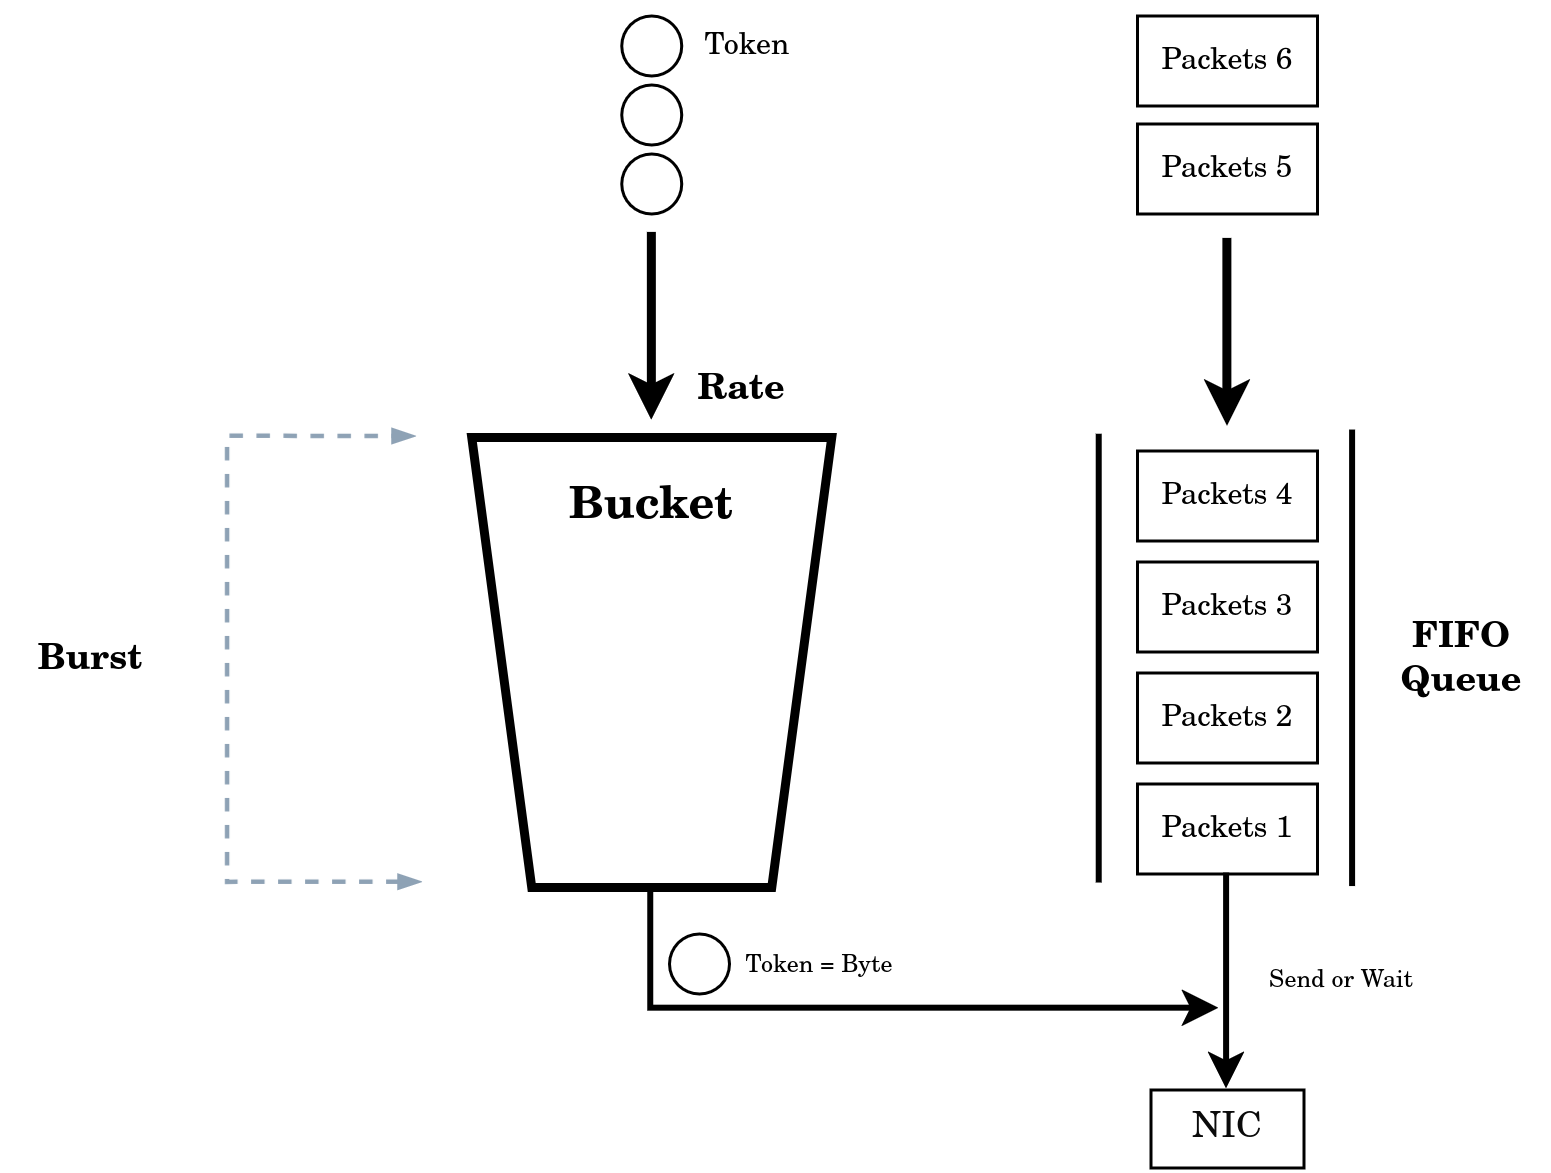
\includegraphics[width=0.7\linewidth]{Images/shaping/tbf.png}
    \caption{Funzionamento di TBF}
\end{figure}

La coda dei pacchetti utilizza una politica \textbf{FIFO} (First In, First Out) e la sua grandezza in byte può essere decisa tramite il parametro \textbf{limit}.
Se piena, i pacchetti successivi vengono scartati direttamente.
\vspace*{0.01\textheight}
\begin{center}
  \begin{tabular}{ |c|c|c| }
    \hline
    \multicolumn{3}{|c|}{\textbf{Parametri comando tc per TBF \cite{tc-tbf}}} \\
    \hline
    \textbf{Parametro} & \textbf{Unità di Misura} & \textbf{Descrizione} \\
    \hline
    rate & $\text{Mbit}/s$ & Velocità di generazione dei tokens. \\
    \hline
    burst & Byte & Capienza del bucket. \\
    \hline
    limit & Byte & Capienza della coda. \\
    \hline
  \end{tabular}
\end{center}

\newpage

\subsection{Hierachical Token Bucket (HTB)}
\begin{defn}[Hierachical Token Bucket]
  Disciplina di accodamento \textbf{classful} disponibile per il controllo del traffico nel comando \texttt{tc}. \\
  Utilizzato per fare traffic shaping controllando la banda in uscita di un interfaccia,
  permettendo di dividere vari flussi tramite l'uso di un albero per creare una \textbf{gerarchia di classi}. 
  L'algoritmo utilizzato per l'elaborazione del traffico è token bucket filter \cite{tc-htb}.
\end{defn}

Ogni classe rappresenta un nodo di un \textbf{albero} e, ad eccezzione della \textbf{radice}, ha una classe \textbf{genitore}.
Questa struttura permette di suddividere ricorsivamente la banda assegnata a una classe tra le sue classi figlie,
ciascuna configurabile con i propri parametri: \textbf{rate} e \textbf{ceil}. \\

\begin{figure}[!htb]
    \centering
    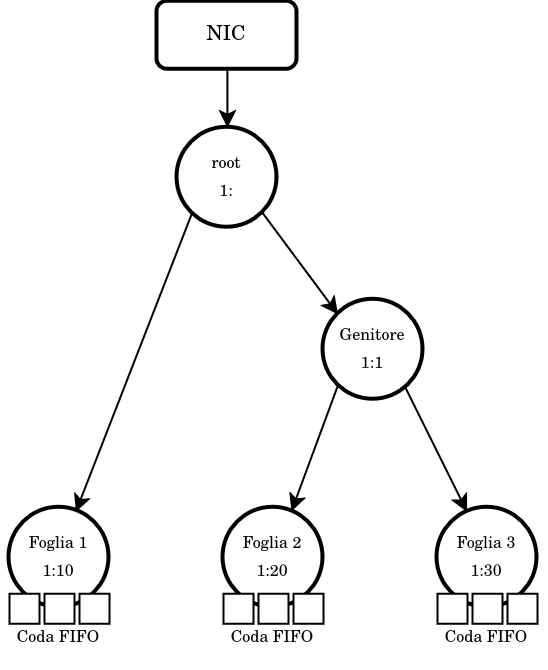
\includegraphics[width=0.5\linewidth]{Images/shaping/htb.png}
    \caption{Gerarchia HTB}
\end{figure}

Le code FIFO di pacchetti in attesa possono essere solo sulle foglie dell'albero, i nodi intermidi non possono accodare.

\subsubsection{Algortimo di Condivisione della Banda}
Tramite questo algoritmo, quando una classe necessita di più banda di quella garantita dal proprio rate,
può prendere in prestito la capacità non utilizzata dalle classi che condividono lo stesso genitore, fino al limite imposto dal proprio ceil.
Il parametro rate indica la banda \textbf{minima} garantita, invecem il parametro ceil indica la banda \textbf{massima} utilizzabile.\\
\vspace*{0.01\textheight}
Una classe genitore conosce la somma della banda effettivamente utilizzata dalle proprie classi figlie e può quindi ridistribuirla a quelle che ne richiedono di più.
Considerando che come algoritmo viene usato token bucket, possiamo includere tutti i casi possibili dei prestiti in tre situazioni diverse \cite{htb-site}:
\begin{itemize}
  \item Il numero di tokens di una classe è sufficiente per inviare immediatamente il pacchetto.
  \item Il numero di tokens di una classe non è sufficiente per inviare immediatamente un pacchetto, ma è possibile chiedere un prestito alla classe genitore, visto che la banda non è satura.
  \item Il numero di tokens di una classe non è sufficiente per inviare immediatamente un pacchetto e non è possibile prendere in prestito ulteriore banda. Il paccheto viene aggiunto alla coda finchè non sarà possibile spedirlo.
\end{itemize}
I parametri utli per l'algoritmo di prestito sono:
\vspace*{0.01\textheight}
\begin{center}
  \begin{tabular}{ |c|c|c| }
    \hline
    \textbf{Parametro} & \textbf{Unità di Misura} & \textbf{Descrizione} \\
    \hline
    rate & $\text{Mbit}/s$ & Velocità minima garantita di generazione dei tokens. \\
    \hline
    burst & Byte & Capienza del bucket. \\
    \hline
    ceil & Mbit$/s$ & Velocità massima possibile di generazione dei tokens. \\
    \hline
    cburst & Byte & Capienza del bucket necessaria quando la \\
     &  & generazione dei tokens è al massimo possibile.\\
    \hline
    quantum & Byte & Byte da inviare prima di passare a un'altra classe. \\
    \hline
  \end{tabular}
\end{center}

\subsubsection{Filtri}
\begin{defn}[Filtro]
  Metodo usato per inserire il pacchetto un una determinata classe in base a diverse caratteristiche, è possibile farli pure tramite il comando \texttt{tc} (traffic control) \cite{tc}.
  Non è l'unico modo pensato per classificare i pacchetti, possono essere usare pure le iptables \cite{iptables}.
\end{defn}
I filtri sono l'oggetto che lega le code code di pacchetti alle classi e possono farlo secondo vari criteri: ip, porte, protocolli, fwmark nel caso vengano usate le iptables e molti altri.

\begin{figure}[!htb]
    \centering
    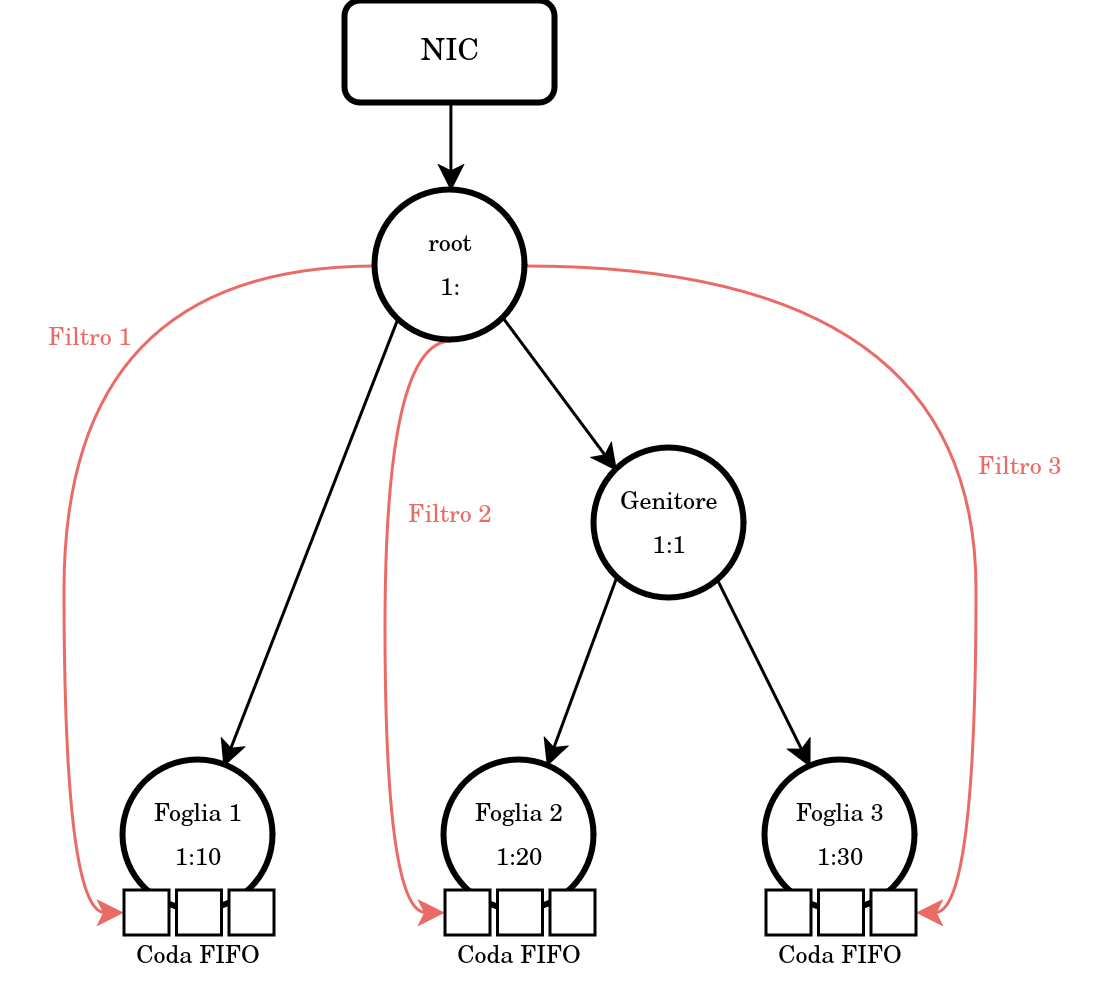
\includegraphics[width=0.6\linewidth]{Images/shaping/filtri.png}
    \caption{Classificazione pacchetti con filtri in HTB.}
\end{figure}
Normalmente la classificazione avviene una sola volta, con i filtri applicati al nodo radice, ma è possibile aggiungere ulteriori filtri nei nodi intermedi.

\newpage
\section{Esempi Reali di Utilizzo}
Il traffic shaping è usato anche i contesti reali. Nei prossimi paragrafi, vorrei mostrare alcuni casi d'uso in cui 
è utile applicare discipline di accodamento come Token Bucke Filter o Hierachical Token Bucket.

\subsection{Limitazione Banda su Backup}
\begin{note}[Scenario]
  Un piccolo ufficio ha una connessione internet condivisa da 20 Mbit/s in upload. Un server esegue un backup automatico verso il cloud in diversi orari della giornata
  e se lasciato libero satura completamente la banda in upload. Si vuole limitare la velocità del traffico il uscita in modo da permettere ai dipendenti di lavorare tranquillamente.
\end{note}

\begin{figure}[!htb]
    \centering
    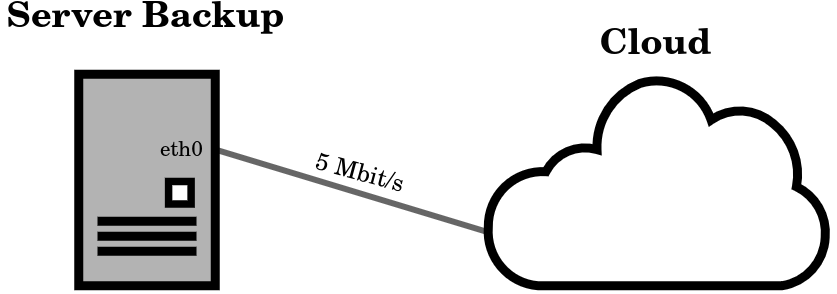
\includegraphics[width=0.6\linewidth]{Images/shaping/Es1.png}
    \caption{Rappresentazione grafica del primo scenario.}
\end{figure}

In questo caso, è possibili limitare il traffico sull'interfaccia di rete del server di backup. 
Ipotizziamo che l'interfaccia sia \texttt{eth0} e che si voglia limitare il traffico a $5$ Mbit$/s$:
\begin{bash}[Comando tc]
  tc qdisc add dev eth0 root tbf rate 5mbit burst 32kb limit 100kb
\end{bash}
Ora, la connessione è correttamente limitata. 

\subsection{Server con Multipli Servizi}
\label{sec:htb}
\begin{note}[Scenario]
  Un server di un'azienda ospita tre servizi per tre clienti diversi: un servizio streaming, un sito web con molto traffico e un servizio di file hosting. \\ 
  La banda totale disponibile e garantita è 100 Mbit/s. Si vuole garantire più banda al cliente del sito web rispetto agli altri due clienti.
  Gli altri due servizi avranno un minimo di banda garantita.
\end{note}

\begin{figure}[!htb]
    \centering
    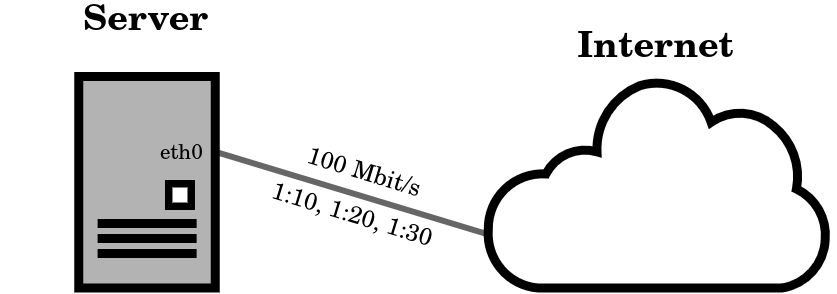
\includegraphics[width=0.6\linewidth]{Images/shaping/Es2.png}
    \caption{Rappresentazione grafica del secondo scenario.}
\end{figure}

In questo caso, con opportuni filtri è possibile inserire i pacchetti nelle code delle classi corrette: \texttt{1:10} per il sito web, \texttt{1:20} per lo streaming e \texttt{1:30} per il file hosting.
\begin{bash}[Classi e parametri con comando tc]
  # Nodo root e genitore
  tc qdisc add dev eth0 root handle 1: htb default 30
  tc class add dev eth0 parent 1: classid 1:1 htb rate 100mbit ceil 100mbit

  # Classe sito web
  tc class add dev eth0 parent 1:1 classid 1:10 htb rate 50mbit ceil 100mbit

  # Classe servizio streaming
  tc class add dev eth0 parent 1:1 classid 1:20 htb rate 35mbit ceil 60mbit

  # Classe servizio file hosting
  tc class add dev eth0 parent 1:1 classid 1:30 htb rate 15mbit ceil 20mbit
\end{bash}
Il nodo genitore ha un minimo e un massimo di banda di 100Mbit/s, che dividerà fra le tre classi, permettendo pure il prestito nel caso fosse possibile. \\
L'ultima cosa che rimane da fare è scrivere i vari filtri che divideranno il traffico nelle opportune code.

\begin{bash}[Filtri con comando tc]
  # Filtri per sito web
  tc filter add dev eth0 protocol ip parent 1:0 prio 1 u32 match ip sport 80 0xffff flowid 1:10
  tc filter add dev eth0 protocol ip parent 1:0 prio 1 u32 match ip sport 443 0xffff flowid 1:10

  # Filtro per servizio streaming 
  tc filter add dev eth0 protocol ip parent 1:0 prio 2 u32 match ip sport <port> 0xffff flowid 1:20

  # Filtro per servizio file hosting
  tc filter add dev eth0 protocol ip parent 1:0 prio 3 u32 match ip sport <port> 0xffff flowid 1:30
\end{bash}
In questo modo, il traffico in uscita con porta sorgente \texttt{80} e porta \texttt{443} (http e https), andrà correttamente nella classe creata per il sito web. 
I pacchetti degli altri due servizi verranno classficati, come fatto in precendenza, in base alla loro porta sorgente. \\ 
Nel comando è stata inserita un diversa priorità per la valutazione dei filtri.

